\documentclass[10pt]{article}
\usepackage[usenames]{color} %used for font color
\usepackage{amssymb} %maths
\usepackage{amsmath} %maths
\usepackage[utf8]{inputenc} %useful to type directly diacritic characters
\usepackage[letterpaper, portrait, margin=1in]{geometry}
\usepackage{graphicx,wrapfig}
\begin{document}
\subsection*{MSDS610 Week 1 Install Hadoop Assignment - Nathan Worsham}
Following the instructions for this week, I started with downloading VirtualBox (currently using a Mac OSX) and CentOS 7 minimal install iso. I chose to stick with minimal install because I am comfortable with using command line only on a machine. 
\par
\raisebox{-.6\height}{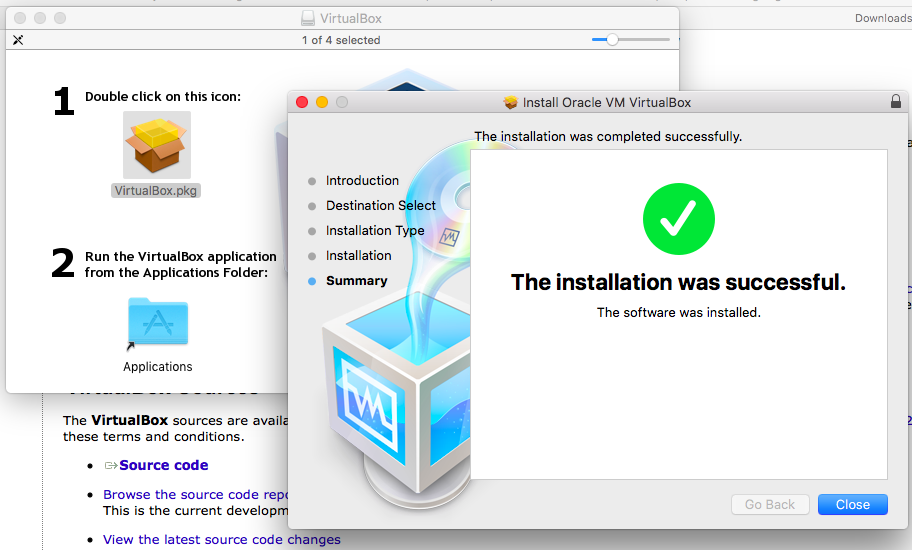
\includegraphics[width=8cm]{virtualbox_install.png}}%
\hfill
\raisebox{-.6\height}{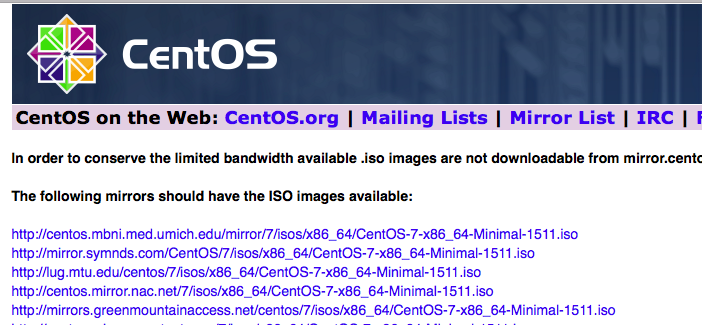
\includegraphics[width=8cm]{minimal_iso_download.png}}%
\par
Next I created a virtual machine named "week1", I chose "Red Hat (64-bit)" for the OS as that is what CentOS is based on and gave it 2 GB of RAM:
\par
\raisebox{-.6\height}{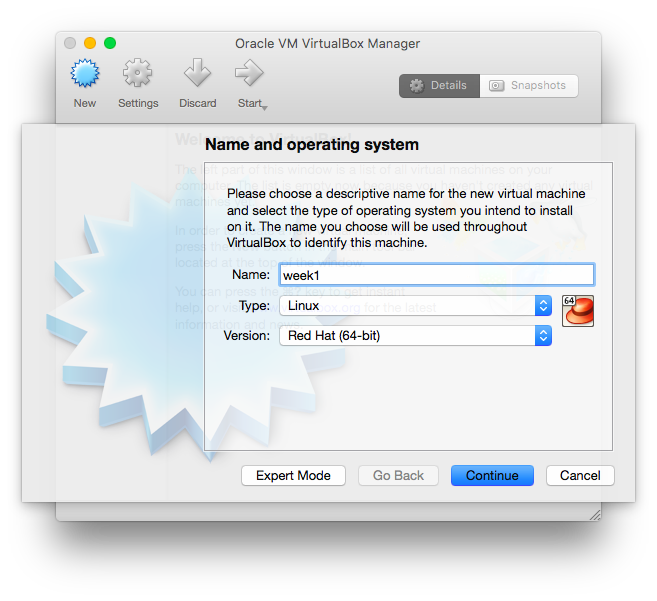
\includegraphics[width=8cm]{vm_setup.png}}%
\hfill
\raisebox{-.6\height}{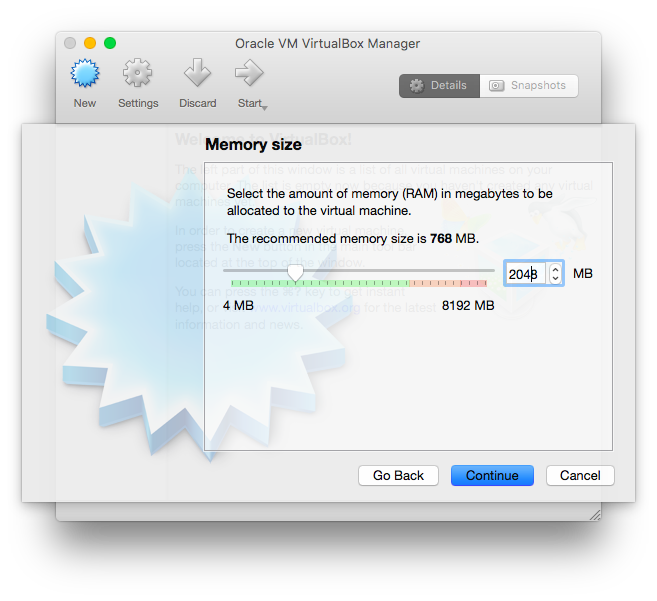
\includegraphics[width=8cm]{mem_setup.png}}%
\par
I chose to use the VMDK format for the disk in case I need to move this to VMWare Player (on my Windows machine) gave the hard drive the 20GB of recommended space. I then enabled the CentOS minimal install ISO to be virtually placed in the cd drive.  
\par
\raisebox{-.6\height}{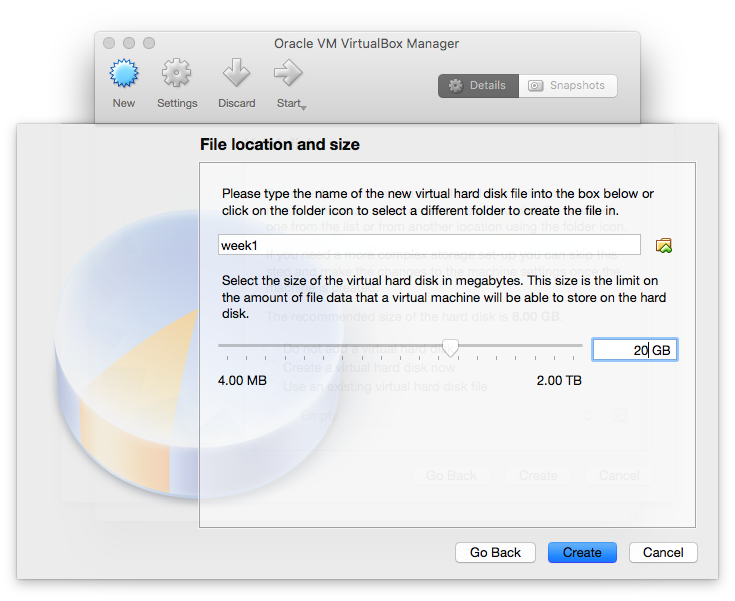
\includegraphics[width=8cm]{disk_setup.png}}%
\hfill
\raisebox{-.6\height}{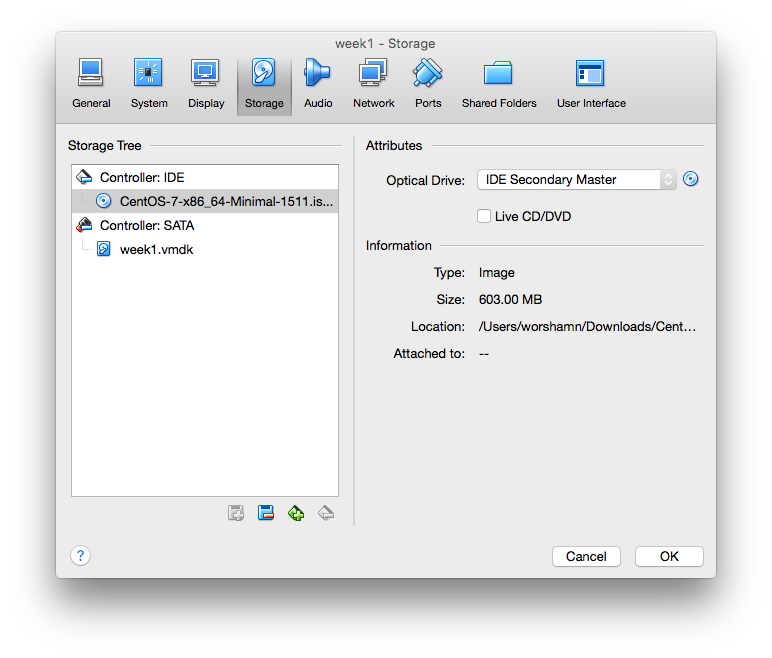
\includegraphics[width=8cm]{iso_setup.png}}%
\par
Logging into the computer was not an issue, but I did run into an issue with what "networking mode" I should use. When I am at home doing the exercises running in Bridged mode, it is not an issue and I can easily both SSH to the virtual machine from the "host" (my Mac laptop) and connect to the internet from the virtual machine. But when I am at my work trying to do the exercises I run into issues. This is because of security in place at my company--802.1x on the wired network, and EAP/TLS on the wireless network. So to allow myself to work on these exercises while at work (on my break time, mind you), I needed to change the configuration. Researching what the different mode options meant from Virtualbox.org (n.d.), I realized I would need to use 2 adapters to accomplish being able to both SSH to the VM and allow the VM out to the Internet given the security constraints. First to get the VM out to the internet I used NAT mode. This hides the VM's IP address behind the host's IP address, but the problem here is that this makes the VM invisible to the host. To solve this I had to add a second adapter running in "Host-Only" mode. To enable this I first had to create a virtual adapter that is a new loopback interface on the host and then assign that adapter the mode. Now I was able to ssh to the VM and get the VM out onto the internet.
\par
\raisebox{-.6\height}{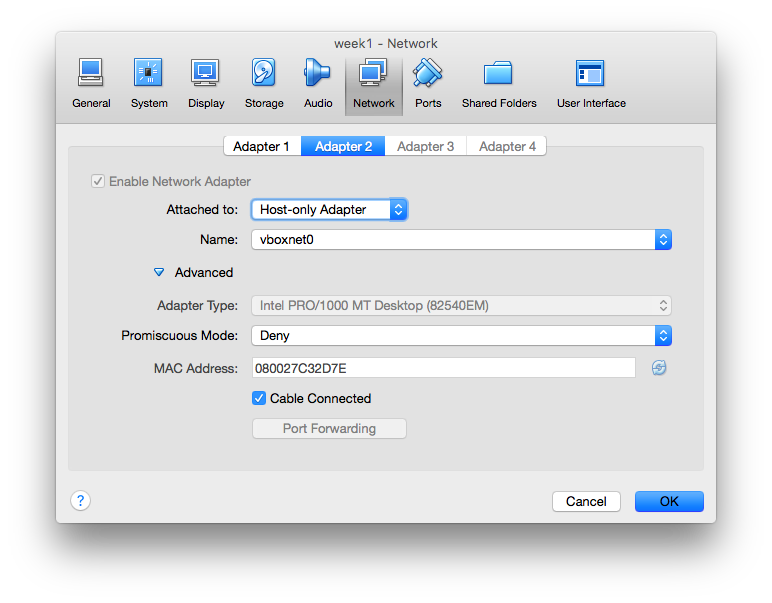
\includegraphics[width=8cm]{host-only.png}}%
\hfill
\raisebox{-.6\height}{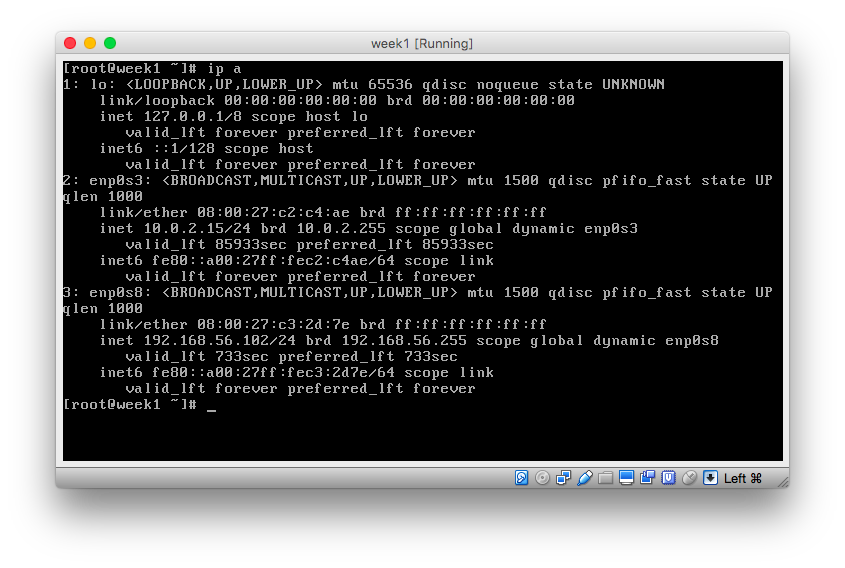
\includegraphics[width=8cm]{ip_a.png}}%
\par
As instructed, I got the latest updates for the OS and then installed wget. Next I was able to use wget to get the java install. I then un-tar'd the file and used \verb|chown| to change the ownership--though I believe root may have already owned it. 
\par
\raisebox{-.6\height}{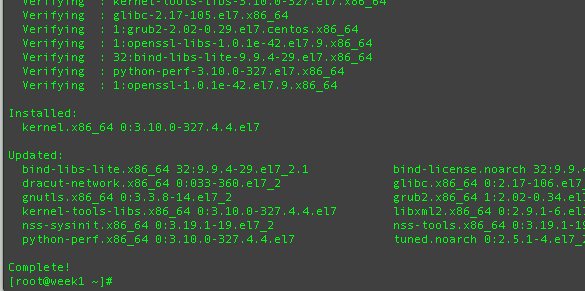
\includegraphics[width=7.7cm]{yum_update.png}}%
\hfill
\raisebox{-.6\height}{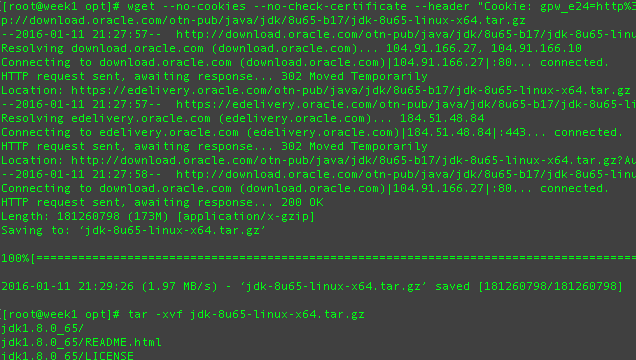
\includegraphics[width=7.7cm]{wget_java.png}}%
\par
I used the \verb|alternatives| command to create symlinks for the various java commands to be used. In my experience, I had only ever just manually created links (with \verb|ln -s|) for programs such as java, I have never even known about the \verb|alternatives| command. It looks like the command keeps basically a note or metadata about the symlink created. When I ran the command 
\begin{verbatim}
alternatives --install /usr/bin/javac javac /opt/jdk1.8.0_65/bin/javac 2
\end{verbatim}
I ran into this error:
\begin{verbatim}
/opt/jdk1.8.0_65/bin/javac has not been configured as an alternative for javac
\end{verbatim}
So I carefully typed out both commands again, this time getting no output, meaning success. Looking through my history using the up arrow, I see an extra character got into my command. In the next section the exercise asks us to create the hadoop user and then later create ssh keys. I am used to creating a user with a home directory to begin with so I did not realize that running just \verb|useradd hadoop| is enough to do so. After running the command I looked at both /etc/passwd and /etc/group files to also find out that the command by default creates a group named hadoop and assigns it to the user.  I then gave the user a password.
\begin{figure}[!h]
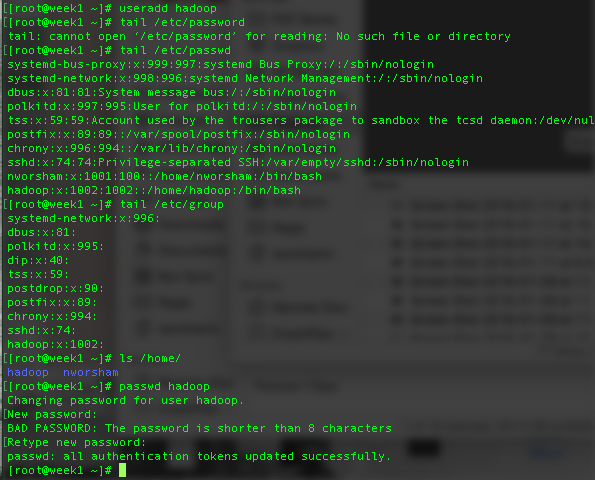
\includegraphics[scale=0.37]{create_user.png}
\centering
\end{figure}\\
Again I am used to setting up ssh keys and copying the public key around for connecting without a password (useful for scripts) from other servers/workstations, but I admit I am a bit confused by copying the public key to the id's own authorized\_keys file. I suppose this is just because this is setting up for another exercise so that perhaps the entire file can be copied is my best guess.
\begin{figure}[!h]
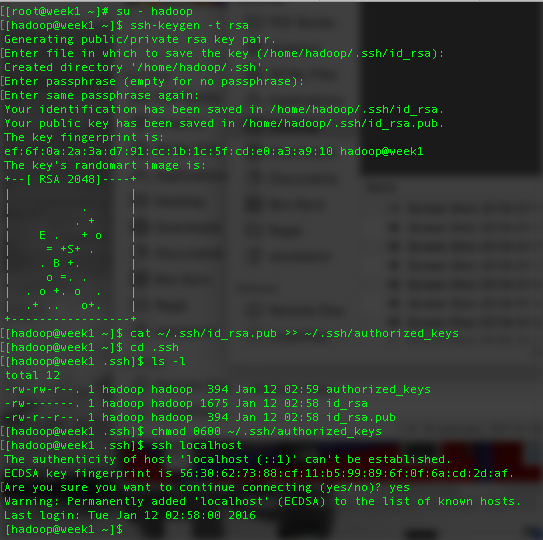
\includegraphics[scale=0.37]{ssh.png}
\centering
\end{figure}\\
I am very comfortable with VI as my editor as I use it day in and day out, mostly because you can always find it installed anywhere. However I went ahead and installed nano and tried it, I can see where someone who is not comfortable or confused by how VI works would like this as a basic editor, but that being said I went back to VI and edited the \verb|.bashrc| profile and completed the remainder of the part 1 assignment.
\pagebreak
\begin{figure}[!h]
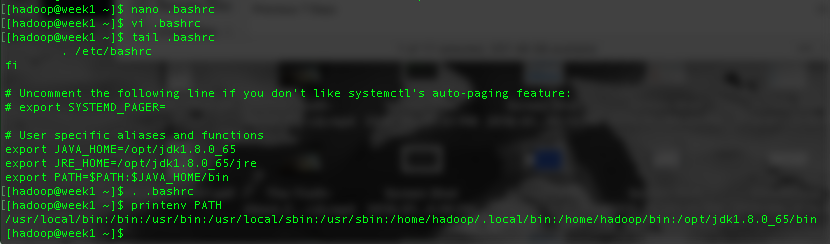
\includegraphics[scale=0.37]{bashrc.png}
\centering
\end{figure}\\
Starting on part 2, I downloaded hadoop and unpacked it. I changed the folder name to \verb|hadoop| but wonder a bit why we wouldn't just set a link or use the alternatives command we previously used. I then set the environment variables:
\begin{figure}[!h]
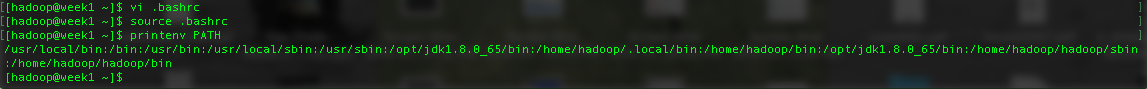
\includegraphics[scale=0.37]{hadoop_path.png}
\centering
\end{figure}\\
Next I used the newly created environment variable \verb|$HADOOP_HOME|, listed directory contents, and updated the \verb|hadoop-env.sh| script to edit its \verb|JAVA_HOME|.
\begin{figure}[!h]
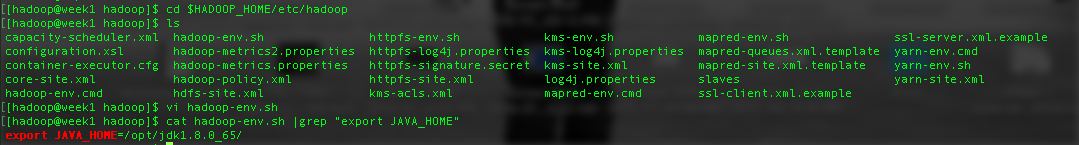
\includegraphics[scale=0.37]{java_home.png}
\centering
\end{figure}\\
After editing the four Hadoop config files, when I tried to run the \verb|hdfs namenode -format| command, I received several errors about the host:
\begin{verbatim}
STARTUP_MSG:   host = java.net.UnknownHostException: week1: week1: unknown error
...
16/01/12 18:06:18 WARN net.DNS: Unable to determine address of the host-falling back to
 "localhost" address
java.net.UnknownHostException: week1: week1: unknown error
...
SHUTDOWN_MSG: Shutting down NameNode at java.net.UnknownHostException: week1: 
week1: unknown error
\end{verbatim}
Off to Google I went with my error message and while Stackoverflow.com (n.d.) did not have the exact answer, it had a similar enough article to make me realize what I needed to do. I'm thinking (but only after the fact) that because I had returned to the exercise after a period of time and did not ssh to localhost from the hadoop user or because I gave my VM a hostname. The error was using my VM's hostname, but since the Stackoverflow.com article pointed at the /etc/hosts file needing a listing for 127.0.0.1 I went there. The file already had the required \verb|localhost| listing, so I just added my VM's hostname (\verb|week1|) to 127.0.0.1 and then the command completed correctly.
\par
\raisebox{-.6\height}{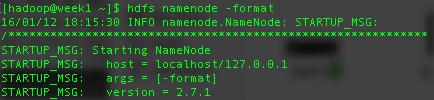
\includegraphics[width=6.5cm]{hdfs_format1.png}}%
\hfill
\raisebox{-.7\height}{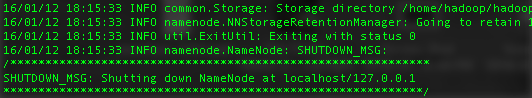
\includegraphics[width=8.5cm]{hdfs_format2.png}}%
\par
Started hdfs and yarn.
\pagebreak
\begin{figure}[!h]
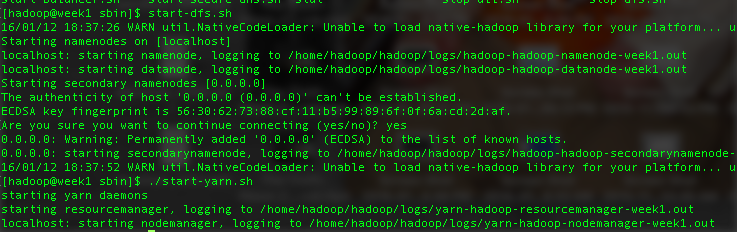
\includegraphics[scale=0.37]{hdfs_yarn.png}
\centering
\end{figure}\\
Started job history server, and confirmed processes with \verb|jps|.
\begin{figure}[!h]
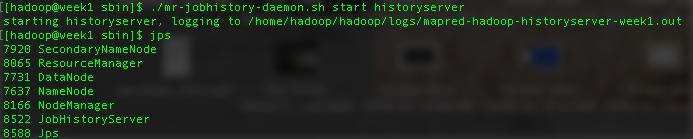
\includegraphics[scale=0.37]{jobhistory.png}
\centering
\end{figure}\\
Trying to run the \verb|firewall-cmd| command, realized firewalld was not installed by both using the command \verb|service firewall status| and opening up the HDFS web interface without configuring anything first.
\par
\raisebox{-.6\height}{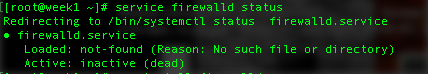
\includegraphics[width=6.5cm]{noFirewall.png}}%
\hfill
\raisebox{-.7\height}{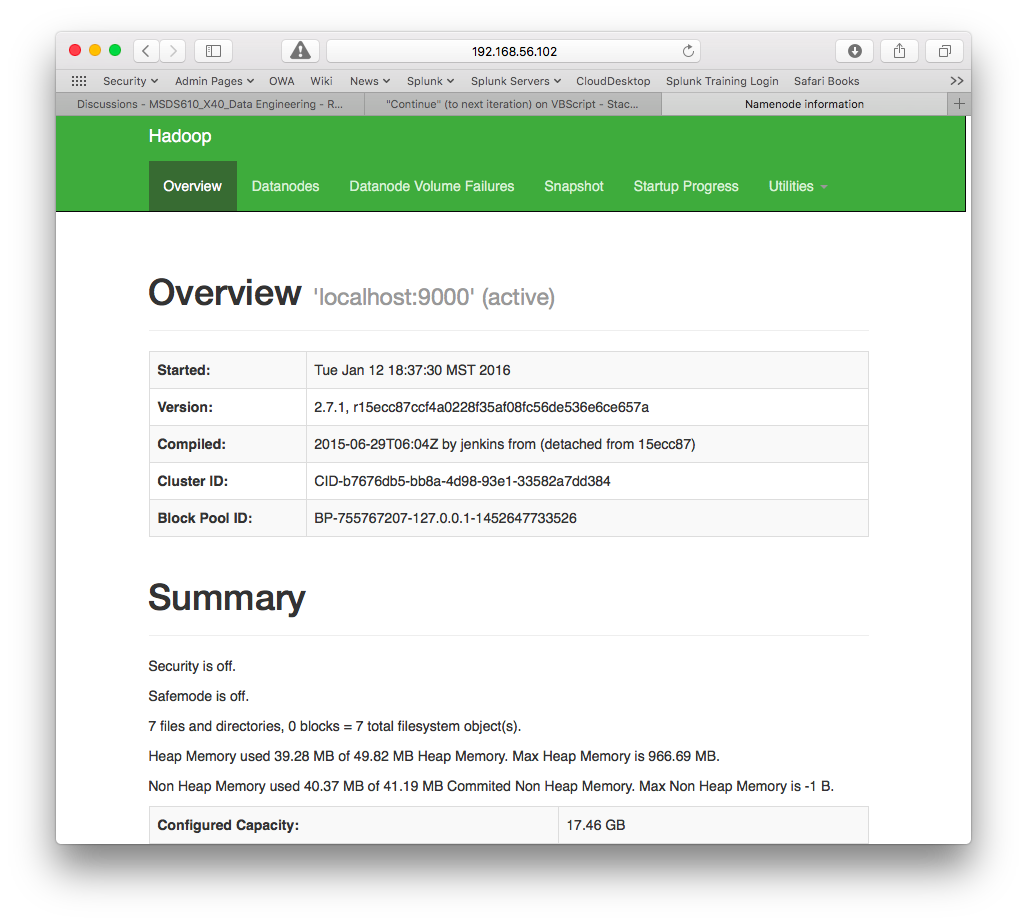
\includegraphics[width=8.5cm]{hdfs_web.png}}%
\par
I went ahead and installed firewalld anyway and confirmed I could no longer get to the web interface for HDFS. So now I opened the ports, however I just used the \verb|--permanent| option and then used \verb|firewall-cmd --reload| to make those changes active. I could then once again get to the HDFS web interface and also tried the YARN interface.
\par
\raisebox{-.6\height}{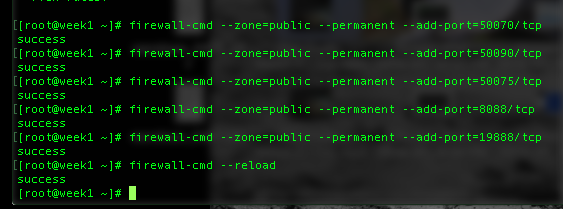
\includegraphics[width=6.5cm]{firewall-cmd.png}}%
\hfill
\raisebox{-.7\height}{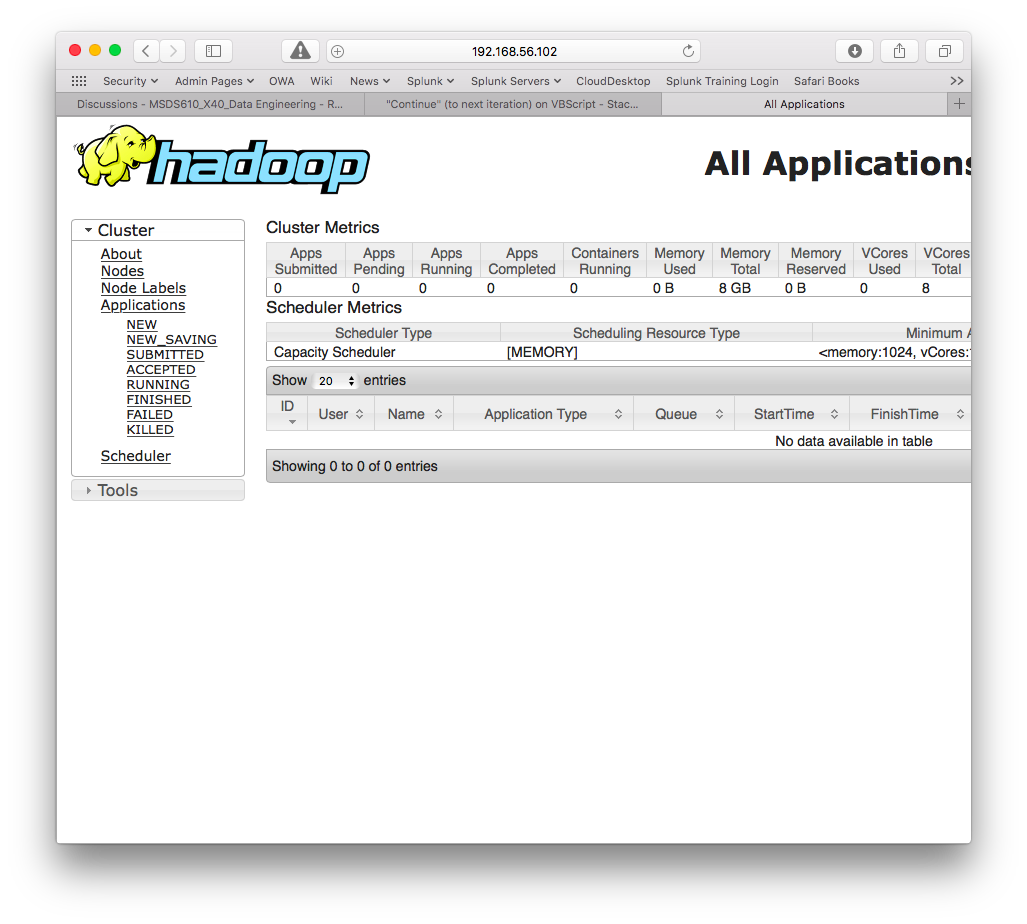
\includegraphics[width=8.5cm]{yarn.png}}%
\par
Last I tested the Hadoop installation but first I went through a Stackoverflow.com (2015) article's solutions to try to figure out how to get rid of the "native-hadoop library" warnings. I finally found that adding the following line to my \verb|.bashrc| file fixed the issue for me.
\begin{verbatim}
export JAVA_LIBRARY_PATH=$HADOOP_HOME/lib/native:$JAVA_LIBRARY_PATH
\end{verbatim}
Showing \verb|head| of the final output file to show I went through the commands. I found on the line about \verb|hadoop-mapreduce-examples-2.7.1.jar|, I had to use the find command to see where this file was located because it gave an error message of \verb|Not a valid JAR: /home/hadoop/hadoop-mapreduce-examples-2.7.1.jar|. Once I gave it the full path of the file it then worked--
\begin{verbatim}
/home/hadoop/hadoop/share/hadoop/mapreduce/hadoop-mapreduce-examples-2.7.1.jar
\end{verbatim}
\begin{figure}[!h]
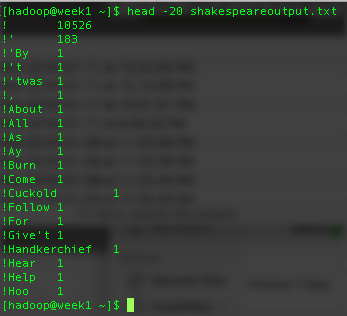
\includegraphics[scale=0.37]{test_hadoop.png}
\centering
\end{figure}
\subsection*{References}
Virtualbox.org, n.d. Chapter 6. Virtual Networking. Retrieved from\\ 
https://www.virtualbox.org/manual/ch06.html\#networkingmodes\\
Stackoverflow.com, 2014. Retrieved from http://stackoverflow.com/questions/24517593/why-hadoop-format-give-out-java-net-unknownhostexception-exception\\
Stackoverflow.com, 2015. Retrieved from http://stackoverflow.com/questions/19943766/hadoop-unable-to-load-native-hadoop-library-for-your-platform-warning
\end{document}
